% -- Encoding UTF-8 without BOM
% -- XeLaTeX => PDF (BIBER)
%% Mainly adapted from: https://www.overleaf.com/latex/templates/friggeri-cv-template/hmnchbfmjgqh

% This thesis proposition template contains topics and guidelines that should help define and select a suitable thesis. 

\documentclass[]{cv-style} % Add 'print' as an option into the square bracket to remove colours from this template for printing. 
 % Add 'italian' as an option into the square bracket to change the date format of the Last Updated Text
\usepackage{polyglossia}
\setdefaultlanguage[]{german}
\usepackage{enumitem}


\sethyphenation[variant=british]{english}{} % Add words between the {} to avoid them to be cut 

\begin{document}

\header{}{Information Sheet} % Your name
\lastupdated

%----------------------------------------------------------------------------------------
%	SIDEBAR SECTION -- In the aside, each new line forces a line break
%----------------------------------------------------------------------------------------

\begin{aside}
% Here include logos of the subjects involved in the research
\section{Lecturer}
%
\color{black}{Prof. A. Wenzel}
%
%\includegraphics[width=2cm]{logos/haw1.png}
%
%
% Contact of the representative
\section{Topic}
Theses
%
%\section{Revision}
%r01
%
\end{aside}

\section{Procedure}

The processing of the topic of the thesis follows the following procedure.

            \begin{figure}[h]
              \colorbox{white}{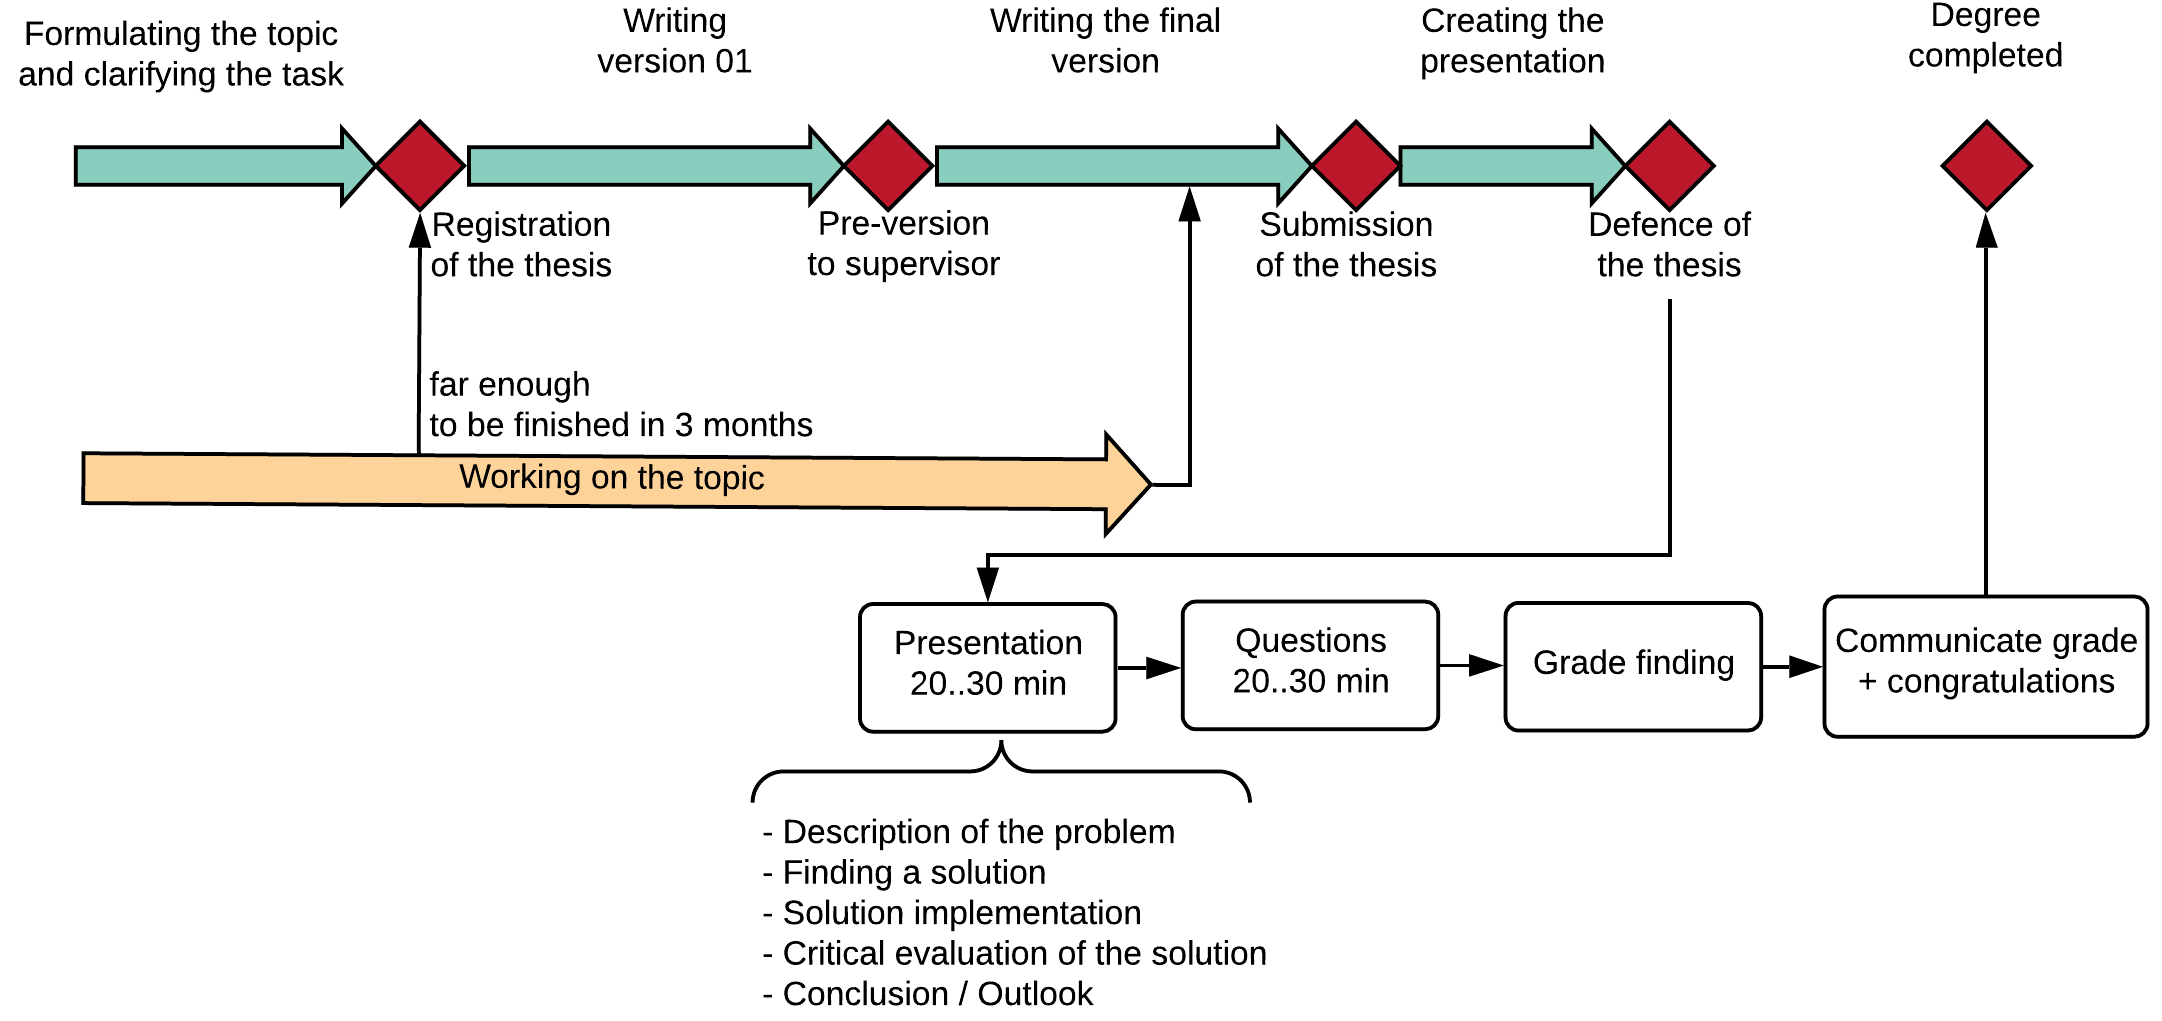
\includegraphics[width=0.8\textwidth]{procedure of the thesis.png}}
            \end{figure}


\bigskip

\section{Meetings}

During the work on the thesis there are several meetings with the supervising professor during which the following must be taken into account

\begin{itemize}
  \item Frequency: 1x per month.
  \item Expectations: Status of work, clarification of problems.
  \item Tools: ongoing Powerpoint presentation by the bachelor student on the status of the work (to be sent to supervisor one evening before).
\end{itemize}
\bigskip

\section{Overview Assessment criteria}
The thesis is assessed on the basis of the following criteria.

%\vspace{-0.7cm}
            \begin{figure}[h]
              \colorbox{white}{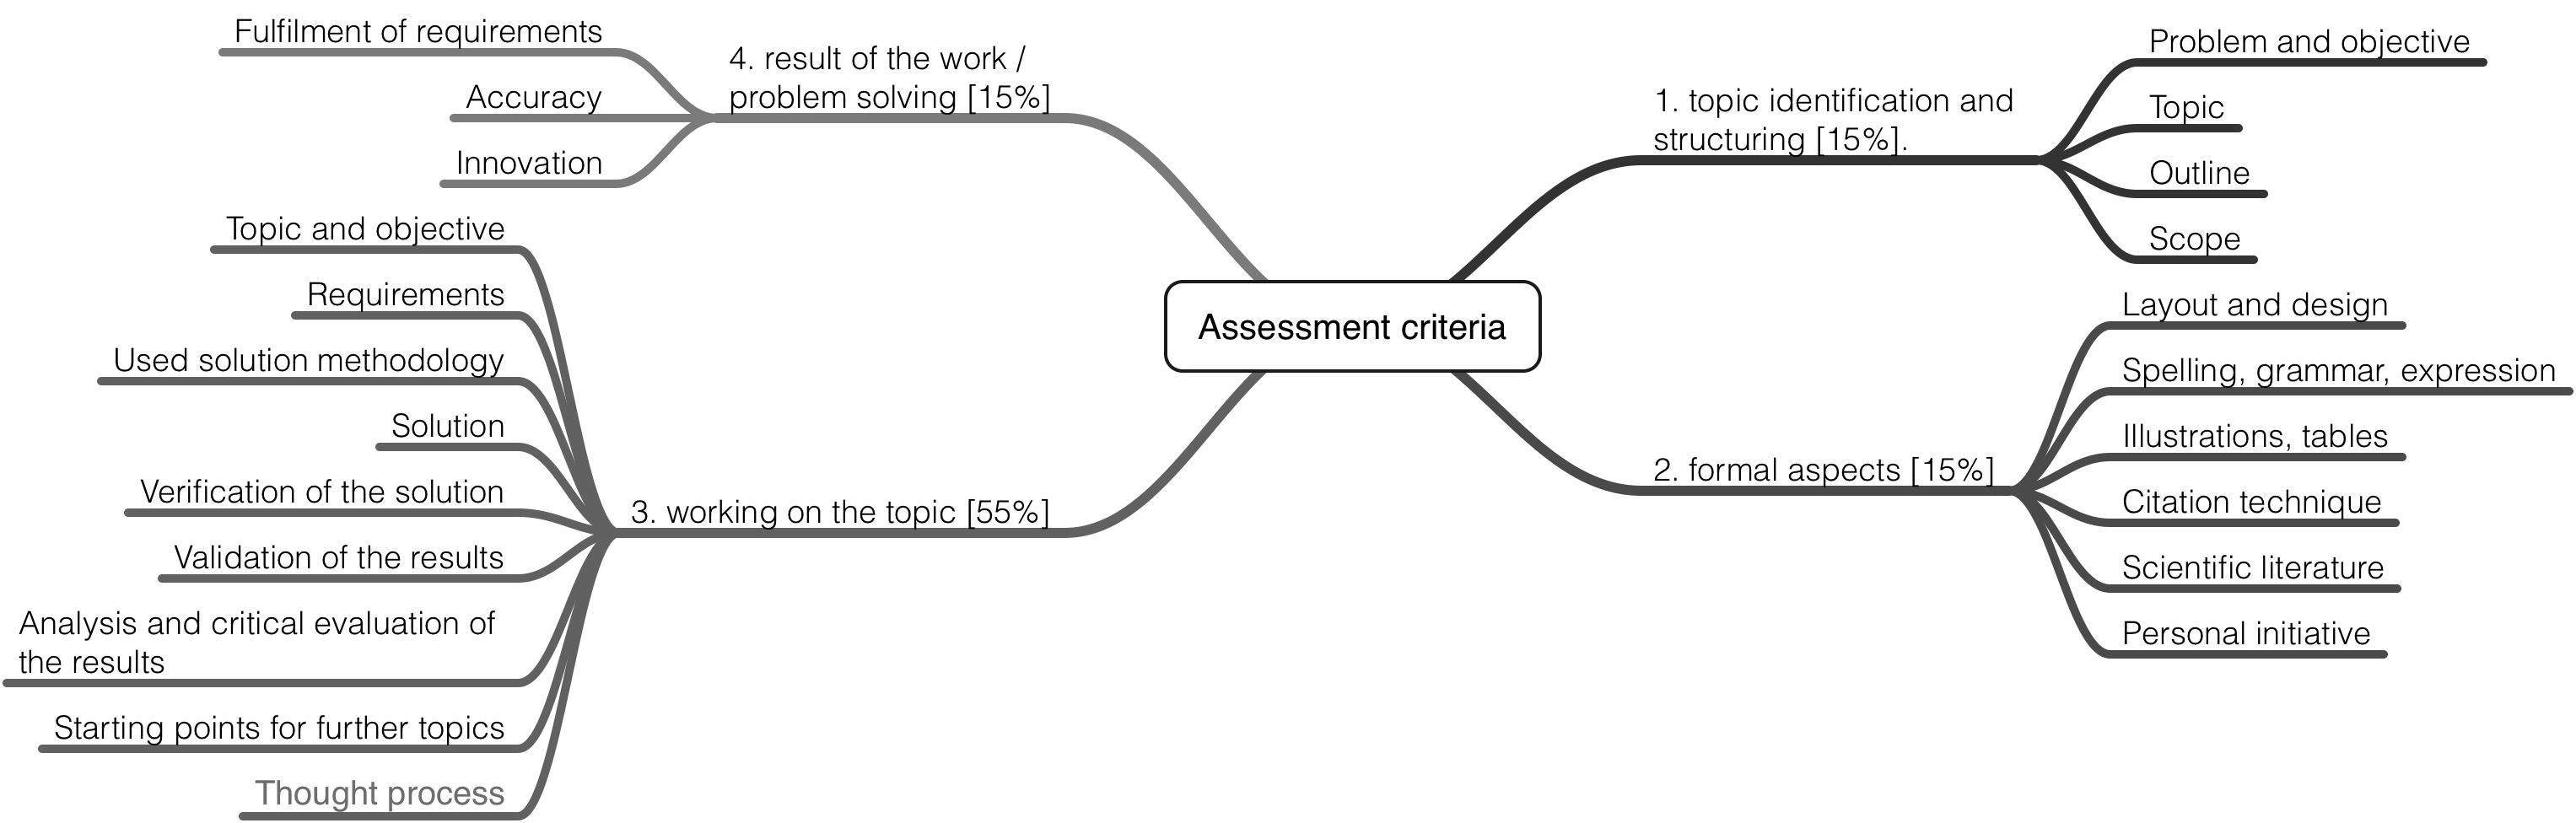
\includegraphics[width=\textwidth]{Assessment criteria.png}}
            \end{figure}
\pagebreak
%------------------------------------------------



\section{Additional information}
 \vspace{-0.2cm}
\color{black}
\textbf{Title of the thesis}
\begin{itemize}[nosep]
	\item No product or company names.
	\item No cryptic abbreviations.
	\item No complicated sentence structure (with brackets and hyphens).
	\item No Matlab in the title.
\end{itemize}
	

\textbf{Writing the thesis}
\begin{itemize}[nosep]
	\item Avoid unclear references (such as "these", "which",...) but write the term in question.
	\item Illustrations support the text, but do not replace it.
	\item Make a reference to the illustration in the text.
\end{itemize}

\textbf{Structure of the thesis} 

A thesis in the field of software development should be structured according to the V-model:
	\begin{figure}[h]
	\centering
              \colorbox{white}{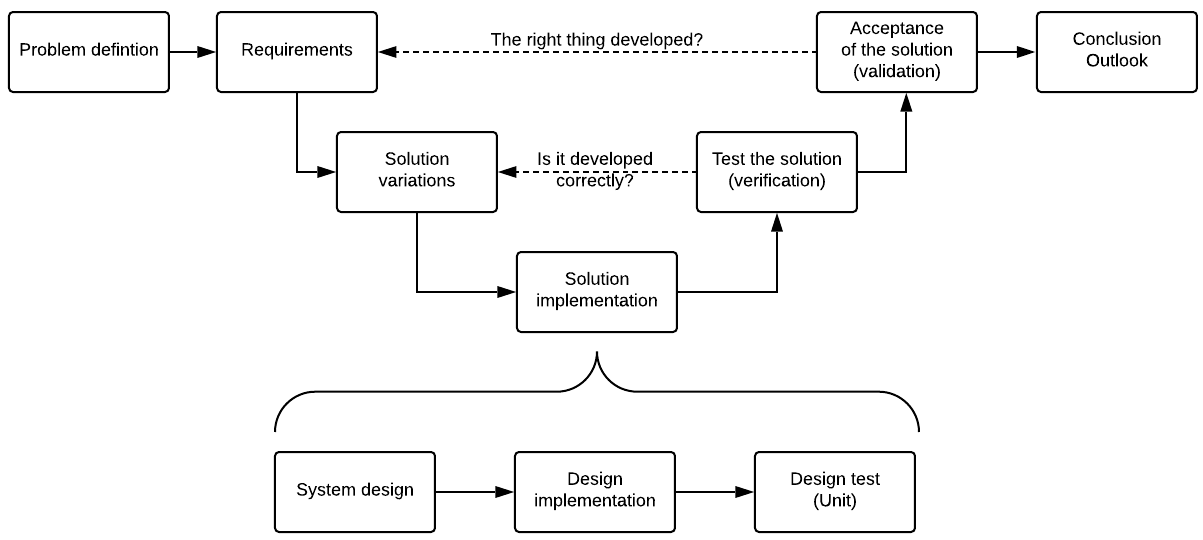
\includegraphics[width=\textwidth]{structure of the thesis.png}}
     \end{figure}

A thesis in the field of data analysis should be structured according to a data analysis process:
	\begin{figure}[h]
	\centering
              \colorbox{white}{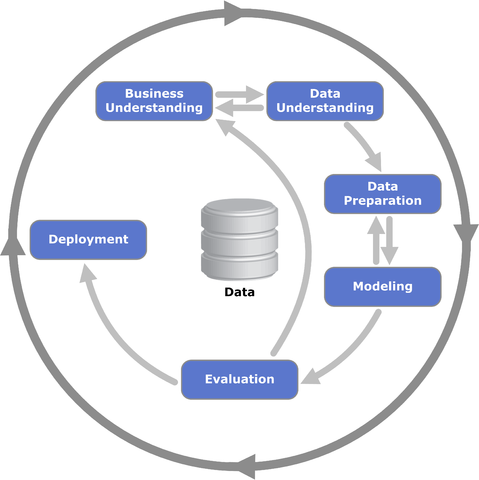
\includegraphics[width=0.4\textwidth]{crispdm.png}}
     \end{figure}

\end{document}